\documentclass{beamer}
\usepackage{beamerthemesplit} % new 
\usepackage[utf8x]{inputenc}
\usepackage[ngerman]{babel} 

\usepackage{epsfig}
\usepackage{amsmath}
\usepackage{placeins}
\usepackage{float}

\usepackage{algorithmic}
\usepackage[linesnumbered,ruled,vlined]{algorithm2e}


\begin{document}
\title{A Hybrid Algorithm for the Partition Coloring Problem (PCP)} 
\author{Gilbert Fritz} 
\date{\today} 

\frame{\titlepage} 

\begin{frame}
\frametitle{Table of contents}

\tableofcontents[hideallsubsections]
\end{frame}


\section{Problem Description} 
\subsection{Partition Coloring Problem}
\frame{\frametitle{Partition Coloring Problem}
\begin{itemize}
\item given $G = (V, E)$
\item let $V_1, V_2,\ldots, V_q$ be a partition of $V$ into $q$ disjoint subsets
\item find a subset $V' \subset V$ such that $|V' \cap V_i| = 1, \forall i = 1, \ldots , q$ (i.e., $V'$ contains one
node from each component $V_i$)
\item find a coloring on the induced graph, such that the chromatic number of the graph induced in $G$ by $V'$ is minimum.  \item Proof of Li and Simha has shown that PCP is $\mathcal{NP}$-complete.
\end{itemize}
}
\frame{\frametitle{Partition Coloring Problem}
\begin{center}
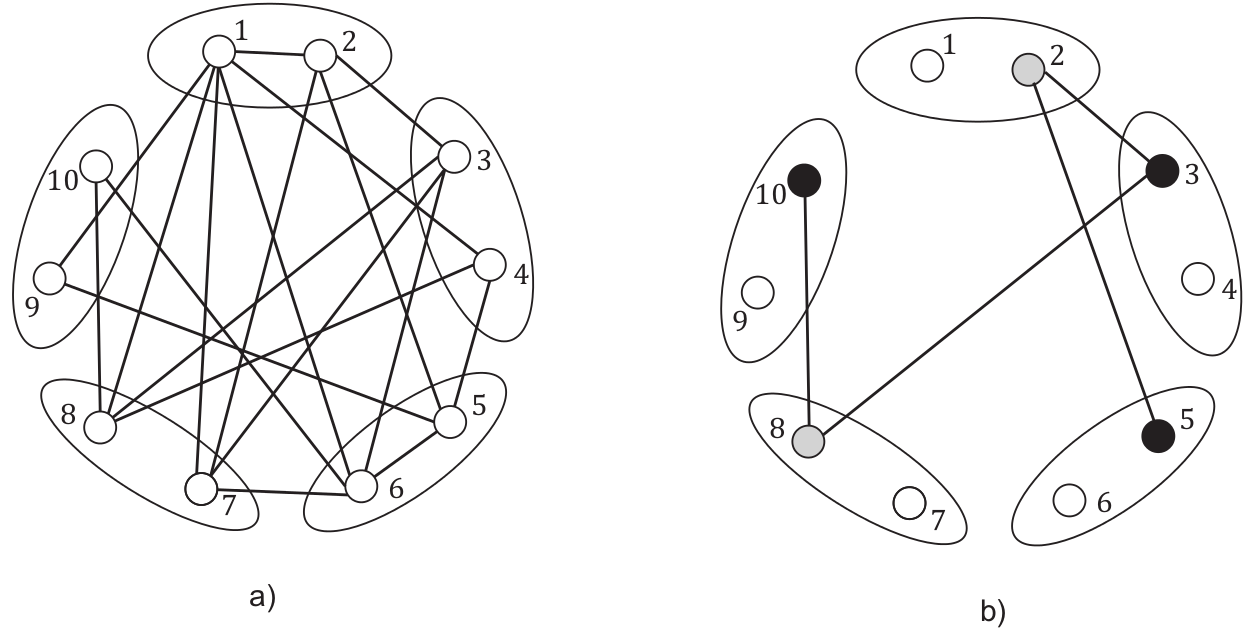
\includegraphics[scale=0.3]{pcp.png}
\end{center}
}

\subsection{Application to min-RWA}
\frame{\frametitle{Routing and Wavelength Assignment}
\begin{itemize}
\item Finding paths
\item Assigning Wavelengths can be modelled as PCP
\end{itemize}
\begin{center}
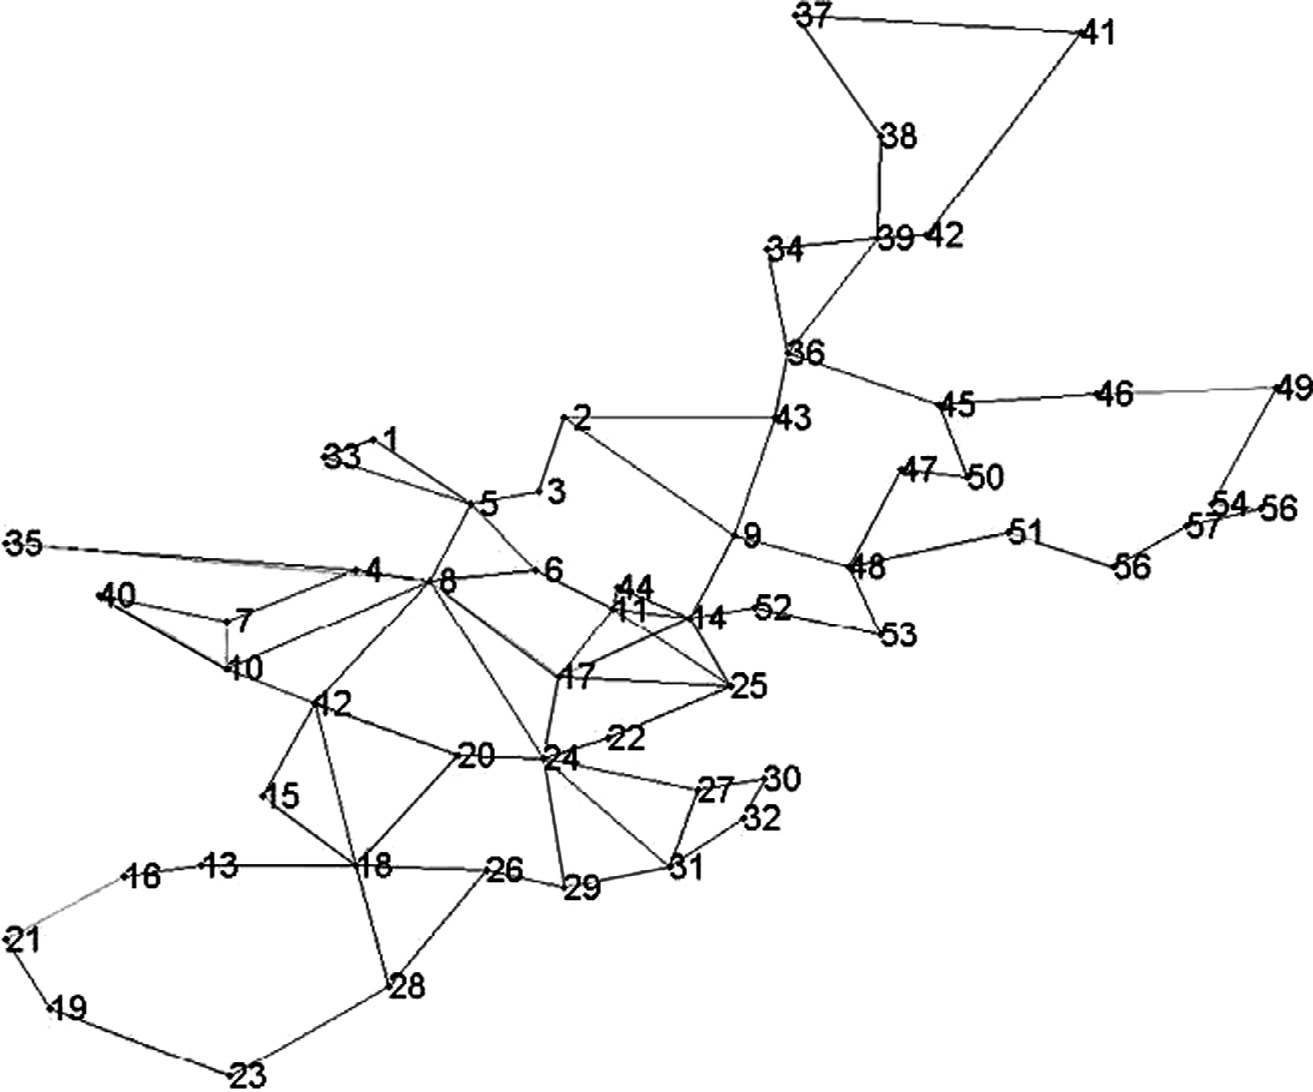
\includegraphics[scale=0.18]{rwa.png}
\end{center}
}


%TODO noch mehr über alle papers schreiben
\section{Previous Works} 
\frame{
\frametitle{Previous Works}
Exact:
\begin{enumerate}
\item Frota, Ribeiro (2010): Branch-And-Cut %algorithm based on a formulation by representative vertices
\item Hoshino, Souza, Frota (2011): Branch-And-Price
\end{enumerate}
Heuristics:
\begin{enumerate}
\item Li, Simha (2000): Group of heuristics based on extensions of classical methods for the vertex coloring problem
\item Noronha, Ribiero (2006): Tabusearch
\item Hu, Raidl, Pop (2013): Memetic algorithm
\end{enumerate}
}

\section{My Approach}
\subsection{Overview}
\frame{\frametitle{Algorithm Overview}
\begin{enumerate}
\item Create initial solution: OneStepCD
\item For each set $U_c$ of clusters of same color $c$: recolor without using $c$ by $\{RANDOM, OneStepCD, ILP1, ILP2\}$
\item Sort the solutions by amount of conflicts.
\item For each solution try to eliminate conflicts by using tabusearch.
\item If all the conflicts could be eliminated, go back to 2, else return the latest feasible solution.
\end{enumerate}
}

\subsection{Initial Solution}
\begin{frame}
\frametitle{Initial Solution: OneStepCD}
  \begin{algorithm}[H]
  \scriptsize
  \KwIn{An uncolored Graph $G=(V,E)$}
  \KwOut{A feasible Coloring $V'$}
  Remove from G all edges $(i,j) \in E$ : $i,j \in V_k$ for some $k=1,\ldots,q$\; 
  Set $V' \gets \emptyset $\;
  \While{$|V'| < q$} {
    Set $X \gets \emptyset $\;
    \For{$k=1,\ldots,q$ : $V_k \cap V'=0$}{
      Set $X \gets X \cup argmin\{CD(i) : i \in V_k\}$\; 
    }
    Set $x \gets argmax\{CD(i) : i \in X \}$\;
    Set $V' \gets V' \cup \{x\}$\;
    Assign the minimum possible colour to x\;
    Remove from G all nodes in $V_{c(x)} \setminus \{x\} $\;
  }
  \Return{$V'$}\;
  \caption{{\sc OneStepCD}}
  \label{algo:osdc}
  \end{algorithm}
\end{frame}

\FloatBarrier
\subsection{Reselecting/Recoloring subgraphs}
\begin{frame}
\frametitle{Random Recoloring}
\begin{enumerate}
\item Nodes are reselected and recolored randomly.
\end{enumerate}

\end{frame}

\frame{\frametitle{Recoloring with OneStepCD}
\begin{algorithm}[H]
\scriptsize
\KwIn{A partial Solution $P$, a number of maximum colours $cmax$ }
\KwOut{A feasible Solution $S$}
Let $U$ be the set of uncolored nodes in $P$\;
Set $S \gets \emptyset$\;
\While{$|U| > 0$} {
  Set $X \gets \emptyset $\;
  \For{ $u \in U$}{
    $X \gets X \cup argmin\{CD(i) : i \in V_{c(u)}\}$\; 
  }
  Set $x \gets argmax\{CD(i) : i \in X \}$\;
  Set $cmin \gets$ the minimum possible colour that can be assigned to x\;
  \If{$cmin \geq cmax$}{
    $cmin \gets$ the color that produces the fewest conflicts.
  }
  Assign $cmin$ to $x$\;
  $S \gets S \cup \{x\}$\;
  $U \gets U \setminus V_{c(x)}$\;
}
\Return{$V'$}\;
\caption{{\sc OneStepCD Recoloring}}
\label{algo:osdc2}
\end{algorithm}
}
\frame{\frametitle{Recoloring with ILP1}

\begin{itemize}
\item Let $Q = {Q_1,\ldots,Q_q}$ be the set of clusters,
\item $C=\{1,\ldots,cmax\}$ the set of allowed colors,
\item $M$ a 3-dimensional array of constants, storing conflicts for each cluster $p \in Q$ and pair $(v \in Q_p, c \in C)$.
\item $E$ denotes the set of edges and $P[v]$ the cluster of node $v$.
\end{itemize}

\begin{equation*}
\scriptsize
\begin{aligned}
& \underset{X}{\text{minimize}} && \sum_{p \in Q}\sum_{v \in Q_p}\sum_{c \in C} X_{pvc} * M_{pvc}                    &&&(1)\\
& \text{subject to} && \sum_{v \in Q_p}\sum_{c \in C} X_{pvc}=1, && \forall p \in Q    &(2)\\
&&& X_{pvc}+X_{quc} \leq 1, && \forall ((p,v),(q,u)) \in E, \forall c \in C     &(3)\\
&&& X_{pvc} \in \{0,1\}, && \forall p \in Q, \forall v \in Q_p, \forall c \in C         &(4)
\end{aligned}
\end{equation*}
}


\frame{\frametitle{Recoloring with ILP2}

\begin{itemize}
\item Let $U$ be the set of uncolored nodes in uncolored clusters
\item and $color[(p,v)]$ the color of the node $v$ in partition $p$
\end{itemize}

\begin{equation*}
\scriptsize
\begin{aligned}
& \underset{Z}{\text{minimize}} && \sum_{p \in Q}\sum_{v \in Q_p}\sum_{c \in C} Z_{pvc}                                              &&&(1)\\
& \text{subject to} && Z_{pvc} \geq X_{quc}, && \forall ((p,v),(q,u))\in E : (p,v) \notin U, (q,u) \in U,\\&&&&& c=color[(p,v)]                                                            &(2)\\
&&& \sum_{v \in Q_p}\sum_{c \in C} X_{pvc}=1, && \forall p \in Q   &(3)\\
&&& X_{pvc}+X_{quc} \leq 1, && \forall ((p,v),(q,u)) \in E, \forall c \in C     &(4)\\
&&& X_{pvc} \in \{0,1\}, && \forall p \in Q, \forall v \in Q_p, \forall c \in C        &(5)
\end{aligned}
\end{equation*}

}

\subsection{Eliminating Conflicts: Tabusearch}
\begin{frame}[fragile]
\frametitle{Tabusearch: Outline}
\begin{enumerate}
\item Let $R$ be the set of clusters that has been recolored before.
\item Initialize $C$ with the set of conflicting clusters not in $R$.
\item Over all cluster in $C$, search for the node-color pair $(n,c)$ that produces the fewest conflicts and is not on the tabulist.
\item Select and color node $n$ with color $c$ and add $(n,c)$ to the tabulist.
\item Remove the cluster of node $n$ from $C$.
\item Add the clusters of all the produced conflicting nodes to set $C$.
\item If $C$ is not empty, go back to step 3.
\end{enumerate}
\end{frame}

%TODO resultate besser darstellen und vergleichen
\section{Results}
\subsection{Instances and Testing Environment}

\frame{\frametitle{Instances and Testing Environment}
\begin{itemize}

%\item Instances of Noronha, Ribiero
%
%\begin{center}
%\begin{tabular}{|c|c|c|c|c|}
%\hline
%\textbf{Instance} & \textbf{Nodes} & \textbf{Clusters} & \textbf{N/Cl} & \textbf{Density} \\
%\hline
%dsjc500.5-1.in & 500 & 500 & 1 & 0.5\\
%\hline
%dsjc500.5-2.in & 1000 & 500 & 2 & 0.5\\
%\hline
%dsjc500.5-3.in & 1500 & 500 & 3 & 0.5\\
%\hline
%dsjc500.5-4.in & 2000 & 500 & 4 & 0.5\\
%\hline
%\end{tabular}
%\end{center}

\item Intel Core i5 DualCore 2.5GHz
\item 8GB Memory
\item Linux Mint 15 (Ubuntu)
\item Java implementation
\item uses single thread
\item cplex 12.5
\item Small instances used by Frota and later Hu
\item Large instance used by Noronha
\end{itemize}
}

\subsection{Instances with different size}

\frame{

\begin{itemize}
\item comparing conflicting nodes per each recoloring  \\
\end{itemize}

\begin{table}
\frametitle{Instances with different size: Conflicting Nodes}
%\caption{hallohallo} 

\resizebox{\columnwidth}{!}{%
\begin{tabular}{|l|l||l||l||l||l|}
\hline
\multicolumn{2}{|l||}{Instance set}&\multicolumn{1}{l||}{Random (10 runs/inst)}&\multicolumn{1}{|l||}{OneStepCD}&\multicolumn{1}{|l||}{ILP1}&\multicolumn{1}{|l|}{ILP2}\\
\cline{1-6}
 nodes & density   & $\overline{cnodes/recoloring}$  & $cnodes/recoloring$ & $cnodes/recoloring$ & $cnodes/recoloring$\\
\hline
20 & 0.5 & 		3.69   & 2.25  	& 1.60  	& \textbf{1.36}\\
40 & 0.5 & 		7.33    & 3.85  & 3.21	  & \textbf{2.29}\\
60 & 0.5 & 		10.21    & 4.99   & 4.21	  & \textbf{2.83}\\
70 & 0.5 & 		11.30    & 5.84	  	& 4.56	  	& \textbf{3.27}\\
80 & 0.5 & 		12.69    & 6.04	 & 4.97 	& \textbf{3.41}\\
90 & 0.5 & 		12.32    & 5.93	  & 4.64	  & \textbf{3.38}\\
100 & 0.5 & 	14.91    & 7.16		  & 5.23	  & \textbf{3.92}\\
120 & 0.5 & 	15.53    & 6.44	  & 5.07	  & \textbf{3.38}\\
\hline
\end{tabular}
}
\begin{tiny}
\textit{$cnodes$ denote the number of conflicting nodes} 
\end{tiny}
\end{table}
}


\frame{

\begin{table}
\frametitle{Instances with different size: Results}

\resizebox{\columnwidth}{!}{%
\begin{tabular}{|l|l||l|l|l||l|l||l|l||l|l|}
\hline
\multicolumn{2}{|l||}{Instance set}&\multicolumn{3}{l||}{Random (10 runs/inst)}&\multicolumn{2}{|l||}{OneStepCD}&\multicolumn{2}{|l||}{ILP1}&\multicolumn{2}{|l|}{ILP2}\\
\cline{1-11}
 nodes & density   & $\overline{obj}$ & $sd$ & $\overline{time}$  & $obj$ & $time$  & $obj$ & $time$  & $obj$ & $time$\\
\hline
20 & 0.5   & \textbf{3.00} & 0.00 & 0.01   & \textbf{3.00} & 0.07  & \textbf{3.00} & 0.11  & \textbf{3.00}  & 0.12\\
40 & 0.5   & \textbf{4.00} & 0.00 & 0.02   & \textbf{4.00} & 0.05  & \textbf{4.00} & 0.14   & \textbf{4.00}  & 0.22\\
60 & 0.5   & \textbf{5.00} & 0.00 & 0.06   & \textbf{5.00} & 0.09  & \textbf{5.00} & 0.25   & \textbf{5.00}  & 0.47\\
70 & 0.5   & \textbf{6.00} & 0.00 & 0.08   & \textbf{6.00} & 0.08  & \textbf{6.00} & 0.21   & \textbf{6.00} & 0.47\\
80 & 0.5   & 6.27 & 0.13 & 0.15  			& \textbf{6.21} & 0.18  & 6.26 & 0.34   			& \textbf{6.21} & 0.75\\
90 & 0.5   & \textbf{7.88} & 0.24 & 0.36  	& 7.91 & 0.38 			 & \textbf{7.88} & 0.59   		& 7.91 & 1.08\\
100 & 0.5   & 7.12 & 0.01 & 0.32   		& 7.22 & 0.32 			 & 7.23  & 0.53   					& \textbf{7.00} & 1.35\\
120 & 0.5   & 8.64 & 0.19 & 0.52   		& 8.64 & 0.64			 & 8.62  & 0.85   					& \textbf{8.60} & 1.89\\
\hline
\end{tabular}
}
\end{table}
}

\frame{

\begin{itemize}
\item Compared to memetic algorithm. Hu, Raidl, Pop (2013)
\item MA2 uses number of colors and number of conflicts for evaluation
\end{itemize}

\begin{table}

\resizebox{\columnwidth}{!}{%
\begin{tabular}{|l|l||l|l||l|l|l||l|l|l|}
\hline
\multicolumn{2}{|l||}{Instance set}&\multicolumn{2}{l||}{B \& C}&\multicolumn{3}{l||}{Random (10 runs/inst)}&\multicolumn{3}{|l|}{MA2}\\
\cline{1-10}
 nodes & density & LB & UB  & $\overline{obj}$ & $sd$ & $\overline{time(s)}$  & $\overline{obj}$ & $sd$ & $\overline{time(s)}$\\
\hline
20 & 0.5  & 3 & 3  & \textbf{3.00} & 0.00 & 0.01   & \textbf{3.00} & 0.00 & 0.14 \\
40 & 0.5  & 4 & 4  & \textbf{4.00} & 0.00 & 0.02   & \textbf{4.00} & 0.00 & 0.60 \\
60 & 0.5  & 5 & 5  & \textbf{5.00} & 0.00 & 0.06   & 5.63 & 0.49 & 2.00 \\
70 & 0.5  & 6 & 6  & \textbf{6.00} & 0.00 & 0.08   & 6.06 & 0.24 & 3.33 \\
80 & 0.5  & 6 & 6  & \textbf{6.27} & 0.13 & 0.15  & 6.94 & 0.29 & 4.90 \\
90 & 0.5  & 6 & 7  & 7.88 & 0.17 & 0.36  & \textbf{7.55} & 0.50 & 7.49 \\
100 & 0.5  & 6 & 7  & \textbf{7.12} & 0.01 & 0.32   & 7.93 & 0.30 & 11.04 \\
120 & 0.5  & 7 & 8  & \textbf{8.64} & 0.19 & 0.52   & 9.22 & 0.43 & 21.05 \\
\hline
\end{tabular}
}
\end{table}
}

\subsection{Instances with different density}

\frame{

\begin{table}
\frametitle{Instances with different density: Conflicting Nodes}
\resizebox{\columnwidth}{!}{%

\begin{tabular}{|l|l||l||l||l||l|}
\hline
\multicolumn{2}{|l||}{Instance set}&\multicolumn{1}{l||}{Random (10 runs/inst)}&\multicolumn{1}{|l||}{OneStepCD}&\multicolumn{1}{|l||}{ILP1}&\multicolumn{1}{|l|}{ILP2}\\
\cline{1-6}
 nodes & density   & $\overline{cnodes/recoloring}$  & $cnodes/recoloring$ & $cnodes/recoloring$ & $cnodes/recoloring$\\
\hline
90 & 0.1 & 		15.71   & 9.50  	& 6.61  	& \textbf{5.65}\\
90 & 0.2 & 		16.70    & 7.99  & 6.36	  & \textbf{4.87}\\
90 & 0.3 & 		15.94    & 7.60   & 5.48	  & \textbf{4.03}\\
90 & 0.4 & 		14.73    & 6.16	  	& 4.75	  	& \textbf{3.41}\\
90 & 0.5 & 		13.51    & 5.93	 & 4.94 	& \textbf{3.43}\\
90 & 0.6 & 		11.78    & 5.20	  & 4.39	  & \textbf{2.84}\\
90 & 0.7 & 		9.60    & 4.61		  & 3.90	  & \textbf{2.44}\\
90 & 0.8 & 		7.70    & 3.66	  & 3.04	  & \textbf{2.05}\\
90 & 0.9 & 		5.56    & 2.69	  & 2.34	  & \textbf{1.74}\\

\hline
\end{tabular}
}
\begin{tiny}
\textit{$cnodes$ denote the number of conflicting nodes} 
\end{tiny}
\end{table}
}

\begin{frame}
\frametitle{Instances with different density: Results}

\begin{table}
\resizebox{\columnwidth}{!}{%
\begin{tabular}{|l|l||l|l|l||l|l||l|l||l|l|}
\hline
\multicolumn{2}{|l||}{Instance set}&\multicolumn{3}{l||}{Random (10 runs/inst)}&\multicolumn{2}{|l||}{OneStepCD}&\multicolumn{2}{|l||}{ILP1}&\multicolumn{2}{|l|}{ILP2}\\
\cline{1-11}
 nodes & density   & $\overline{obj}$ & $sd$ & $\overline{time(s)}$  & $obj$ & $time(s)$  & $obj$ & $time(s)$  & $obj$ & $time(s)$\\
\hline
90 & 0.1   & \textbf{3.00} & 0.00 & 0.02   & \textbf{3.00} & 0.11  	& \textbf{3.00} & 0.16 & 	\textbf{3.00} & 0.36\\
90 & 0.2   & \textbf{3.80} & 0.15 & 0.03   & \textbf{3.80} & 0.06  	& \textbf{3.80} & 0.15 & 	\textbf{3.80} & 0.51\\
90 & 0.3   & \textbf{5.00} & 0.00 & 0.06   & \textbf{5.00} & 0.06  	& \textbf{5.00} & 0.17 & 	\textbf{5.00} & 0.43\\
90 & 0.4   & \textbf{6.00} & 0.00 & 0.11   & \textbf{6.00} & 0.11  	& \textbf{6.00} & 0.26 & 	\textbf{6.00} & 0.59\\
90 & 0.5   & \textbf{7.00} & 0.00 & 0.18   & \textbf{7.00} & 0.19  	& \textbf{7.00} & 0.39  & 	\textbf{7.00} & 0.84\\
90 & 0.6   & 8.28 & 0.15 & 0.31   			 & 8.40 & 0.36  			& \textbf{8.20} & 0.58 	& 	8.40 & 1.03\\
90 & 0.7   & \textbf{10.00} & 0.00 & 0.45   & \textbf{10.0} & 0.45  	& \textbf{10.00} & 0.73   	& \textbf{10.00} & 1.25\\
90 & 0.8   & \textbf{12.05} & 0.01 & 0.80   & 12.20 & 0.77  			& 12.20 & 1.16 &				12.20 & 1.83\\
90 & 0.9   & \textbf{15.80} & 0.15 & 1.23   & \textbf{15.80} & 1.26  	& \textbf{15.80} & 1.62 &	\textbf{15.80} & 2.27\\
\hline
\end{tabular}
}
\end{table}
\end{frame}

\frame{
\frametitle{Instances with different density: Compared}

\begin{itemize}
\item Compared to memetic algorithm. Hu, Raidl, Pop (2013)
\item MA2 uses number of colors and number of conflicts for evaluation
\end{itemize}

\begin{table}
\resizebox{\columnwidth}{!}{%
\begin{tabular}{|l|l||l|l||l|l|l||l|l|l|}
\hline
\multicolumn{2}{|l||}{Instance set}&\multicolumn{2}{l||}{B \& C}&\multicolumn{3}{l||}{Random (10 runs/inst)}&\multicolumn{3}{|l|}{MA2}\\
\cline{1-10}
 nodes & density & LB & UB  & $\overline{obj}$ & $sd$ & $\overline{time(s)}$  & $\overline{obj}$ & $sd$ & $\overline{time(s)}$\\
\hline
90 & 0.1  & 2 & 3  & \textbf{3.00} & 0.00 & 0.02   & 3.09 & 0.29 & 1.37 \\
90 & 0.2  & 3 & 4  & \textbf{3.80} & 0.15 & 0.03   & 4.41 & 0.49 & 3.24 \\
90 & 0.3  & 4 & 5  & \textbf{5.00} & 0.00 & 0.06   & 5.52 & 0.56 & 4.90 \\
90 & 0.4  & 5 & 6  & \textbf{6.00} & 0.00 & 0.11   & 6.79 & 0.83 & 6.54 \\
90 & 0.5  & 6 & 7  & \textbf{7.00} & 0.00 & 0.18  & 7.55 & 0.50 & 7.49 \\
90 & 0.6  & 8 & 8  & \textbf{8.28} & 0.15 & 0.31  & 10.50 & 0.87 & 11.95 \\
90 & 0.7  & 10 & 10  & \textbf{10.00} & 0.00 & 0.45   & 12.39 & 1.12 & 14.83 \\
90 & 0.8  & 12 & 12  & \textbf{12.05} & 0.14 & 0.80   & 15.18 & 0.80 & 20.98 \\
90 & 0.9  & 16 & 16  & \textbf{15.80} & 0.15 & 1.23   & 17.27 & 0.98 & 45.75 \\
\hline
\end{tabular}
}
\end{table}
}

\subsection{Large instances}


\frame{

\begin{table}
\frametitle{Large instances: Conflicting Nodes}
\resizebox{\columnwidth}{!}{%

\begin{tabular}{|l|l||l||l||l||l|}
\hline
\multicolumn{2}{|l||}{Instance set}&\multicolumn{1}{l||}{Random (10 runs/inst)}&\multicolumn{1}{|l||}{OneStepCD}&\multicolumn{1}{|l||}{ILP1}&\multicolumn{1}{|l|}{ILP2}\\
\cline{1-6}
 nodes & density   & $\overline{cnodes/recoloring}$  & $cnodes/recoloring$ & $cnodes/recoloring$ & $cnodes/recoloring$\\
\hline
500 & 0.5 & 		35.13   & 7.89  	& 7.88  	& \textbf{5.02}\\
1000 & 0.5 & 		39.87    & 9.15  & 7.74	  & \textbf{5.15}\\
1500 & 0.5 & 		44.67    & 11.52   & 8.12	  & \textbf{6.02}\\
2000 & 0.5 & 		46.81    & 12.29	  	& 4.75	  	& \textbf{6.42}\\

\hline
\end{tabular}
}
\begin{tiny}
\textit{$cnodes$ denote the number of conflicting nodes} 
\end{tiny}
\end{table}
}

\begin{frame}
\frametitle{Large Instances: Results}

\begin{table}
\resizebox{\columnwidth}{!}{%
\begin{tabular}{|l|l||l|l|l||l|l|l||l|l|l||l|l|l|}
\hline
\multicolumn{2}{|l||}{Instance set}&\multicolumn{3}{l||}{Random (10 runs/inst)}&\multicolumn{3}{|l||}{OneStepCD}&\multicolumn{3}{|l||}{ILP1}&\multicolumn{3}{|l|}{ILP2}\\
\cline{1-14}
 nodes & density   & $\overline{obj}$ & $sd$ & $\overline{time(s)}$  & $obj$ & $sd$ & $time(s)$  & $obj$ & $sd$ & $time(s)$  & $obj$ & $sd$ & $time(s)$\\
\hline
500 & 0.5    & 53.6 & 0.0 & 18.011   			& \textbf{53.0} & 0.0 & 19.91  & \textbf{53.0} & 0.0 & 29.87 & \textbf{53.0} & 0.0 & 118.90\\
1000 & 0.5   & \textbf{48.0} & 0.0 & 67.74   	& \textbf{48.0} & 0.0 & 76.68  & \textbf{48.0} & 0.0 & 107.20 & \textbf{48.0} & 0.0 & 637.36\\
1500 & 0.5   & 45.4 & 0.0 & 202.99   			& \textbf{45.0} & 0.0 & 175.14 & 46.0 & 0.0 & 244.90 			&  \textbf{45.0} & 0.0 & 3005.96\\
2000 & 0.5   & \textbf{43.8} & 0.0 & 316.90   & 44.0 & 0.0 & 289.03  			& 44.0 & 0.0 & 473.30 				& 44.0 & 0.0 & 7637.26\\
\hline
\end{tabular}
}
\end{table}
\end{frame}

\frame{
\frametitle{Large instances: Compared}

\begin{itemize}
\item Compared to Local Search. Noronha, Ribiero (2006)
\end{itemize}

\begin{table}
\resizebox{\columnwidth}{!}{%
\begin{tabular}{|l|l||l|l|l|l||l|l|l|}
\hline
\multicolumn{2}{|l||}{Instance set}&\multicolumn{4}{l||}{Random (10 runs/inst)}&\multicolumn{3}{|l|}{Nohora (10 runs/inst)}\\
\cline{1-9}
 nodes & density & $min$ & $avg$ & $max$ & $\overline{time(s)}$  & $min$ & $avg$ & $max$\\
\hline
500 & 0.5  & 53 & 53.6 & 54 & 18.01  	& 51 & \textbf{51.3} & 52 \\
1000 & 0.5  & 48 & 48.0 & 48 & 67.74   & 45 & \textbf{45.9} & 46 \\
1500 & 0.5  & 45 & 45.4 & 46 & 202.99   & 43 & \textbf{43.2} & 44 \\
2000 & 0.5  & 43 & 43.8 & 44 & 316.90   & 42 & \textbf{42.0} & 42 \\
\hline
\end{tabular}
}
\end{table}
}



\section{Summary}
\subsection{Summary}
\frame{
\frametitle{Summary}
Main insight:
\begin{itemize}
\item optimizing the number of conflicting nodes does not lead to better results
\end{itemize}
Advantages:
\begin{itemize}
\item low calculation time when recoloring randomly or using OneStepCD
\item good results compared to other heuristical methods
\end{itemize}
Disadvantages:
\begin{itemize}
\item Noronha and Ribiero's tabusearch search still performs slightly better
\end{itemize}
}

\subsection{Future works}
\begin{frame}
\frametitle{Future works}
\begin{itemize}
\item All node-color-combinations from all recently recolored clusters could be put on the tabulist for a number of iterations
\item adapt size of tabulist to instances more individually
\item try first improvement strategy
\end{itemize}
\end{frame}

\subsection{Discussion}
\frame{
\frametitle{Discussion}
\begin{itemize}
\item Questions?
\end{itemize}
}


\begin{frame}[fragile]
\frametitle{Pseudocode Tabusearch}
\includegraphics[scale=0.25]{tabusearch.png}
\end{frame}


%\begin{frame}
%\bibliographystyle{unsrt}   % this means that the order of references
%			    % is dtermined by the order in which the
%			    % \cite and \nocite commands appear
%\bibliography{pcp}  % list here all the bibliographies that
%\end{frame}

\end{document}
